\documentclass[tikz]{standalone}

\usepackage{pgfplots}
\pgfplotsset{compat=1.15}
\usepackage{mathrsfs}
\usetikzlibrary{arrows,calc}
\usepackage{tkz-euclide}
\pagestyle{empty}

\definecolor{AngleClr}{rgb}{0,0.39215686274509803,0}
\definecolor{ShapeClr}{rgb}{0.6,0.2,0}
\definecolor{BlueSqr}{RGB}{5,81,163}
\definecolor{SecondAngleClr}{RGB}{176, 53, 19}


\begin{document}

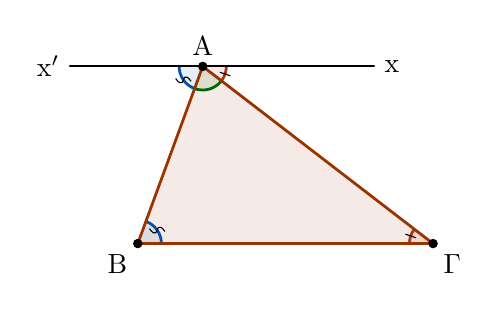
\begin{tikzpicture}[scale=.75]
\tkzSetUpLine[line width=1pt,color=black]
\tkzSetUpPoint[fill=black]

\tkzDefPoints{0/0/B,1.1/3/A,5/0/C}
\tkzDefPoints{-1.15/3/x',4/3/x}

\tkzDefMidPoint(A,B) \tkzGetPoint{MC}
\tkzDefMidPoint(A,C) \tkzGetPoint{MB}

\tkzDefPointsBy[symmetry=center MB](MC){}

\tkzFillPolygon[fill=ShapeClr,fill opacity=0.1](C,B,A)

\tkzFillAngle[fill=AngleClr,size=.4,fill opacity=0.1](B,A,C)
\tkzMarkAngle[line width=1pt,color=AngleClr,size=.4](B,A,C)

\tkzFillAngles[fill=BlueSqr,size=.4,fill opacity=0.1](C,B,A x',A,B)
\tkzMarkAngles[mark=s,mksize=2,line width=1pt,color=BlueSqr,size=.4](C,B,A x',A,B)

\tkzFillAngles[fill=SecondAngleClr,size=.4,fill opacity=0.1](A,C,B C,A,x)
\tkzMarkAngles[mark=|,mksize=2,line width=1pt,color=SecondAngleClr,size=.4](A,C,B C,A,x)

\tkzDrawSegments[line width=0.75pt,color=black](x,x')

\tkzDrawPolygon[color=ShapeClr](A,B,C)
\tkzDrawPoints[size=3](A,B,C)

\tkzLabelPoint[above](A){$\rm A$}
\tkzLabelPoint[below left](B){$\rm B$}
\tkzLabelPoint[below right](C){$\rm \Gamma$}

\tkzLabelPoint[left](x'){$\rm x'$}
\tkzLabelPoint[right](x){$\rm x$}

\end{tikzpicture}

\end{document}
